\section{Distributed Acoustic Sensing}
\label{back:das}

\acrfull{das} is a type of sensing technology that uses fiber optic cables to measure strain and vibrations along their length. By employing specialized optoelectronic devices, \acrshort{das} systems can detect and measure acoustic disturbances over vast distances with high spatial and temporal resolution. This technology is widely used for monitoring conditions within geophysical environments. Some of the usecases of \acrshort{das} at \acrshort{cgf} include

\begin{itemize}
    \item Movement of traffic
    \item Detection of landslides
    \item Observation of Whales outside Svalbard
    \item Seismic activity detection
\end{itemize}


\begin{figure}[!h]
    \centering
    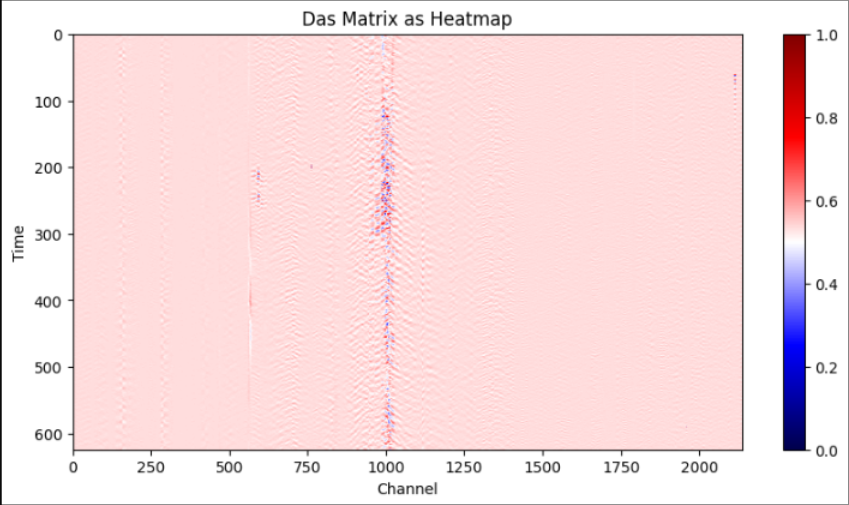
\includegraphics[width=0.7\linewidth]{figures/das_example.png}
    \caption{DAS data frame example}
    \label{fig:dasframe-ex}
\end{figure}

\subsection{Numerical analysis}

\acrshort{das} data can be stored in several different file formats. Data stored in \acrshort{hdf5} files have the advantage of storing additional metadata beside it and is ideal for complex datasets requiring extensive contextual information. Other formats such as TDMS are also structured around hierarchical data \cite{10.1145/800196.805973}, and is often used for storing \acrshort{das} data. Regardless of the chosen format, certain metadata are crucial for effectively handling and interpreting DAS data:

\textbf{Timestamps} is used for temporal alignment and analysis

\textbf{Gauge length} is the spatial resolution of measurements

\textbf{Channel decimation} stores information on spatial sampling. Not all channels along the total measurement is stored, and so to understand the location of a signal, the gauge length in combination with the channel decimation tells us the exact distance from the start of the measurement.

\textbf{Sample Rate} is the temporal resolution of the data, and is measured in hertz.

\acrshort{das} data itself is stored as a matrix, usually where the axis represent time and signal channels.

\begin{table}[!h]
\centering
\begin{equation*}
\mathbf{X} = \begin{bmatrix}
x_{1,1} & x_{1,2} & \cdots & x_{1,n-1} & x_{1,n} \\
x_{2,1} & x_{2,2} & \cdots & x_{2,n-1} & x_{2,n} \\
\vdots & \vdots & \ddots & \vdots & \vdots \\
x_{t-1,1} & x_{t-1,2} & \cdots & x_{t-1,n-1} & x_{t-1,n} \\
x_{t,1} & x_{t,2} & \cdots & x_{t,n-1} & x_{t,n}
\end{bmatrix}
\end{equation*}
\label{fig:dasmatrix}
\end{table}

In the matrix $\textbf{X}$ above, $t$ denotes the max amount of recordings for the file; for one second this would be equal to the sample rate. $n$ is the amount of channels stored. To process this data as fast as possible, it is important to consider which memory alignment the programming language of choice uses. In Julia, MatLab and Fortran, memory is stored in column-major order, while in most other languages, memory is stored in a row-major order. 